\documentclass[a4paper]{article}
\usepackage[utf8]{inputenc}
\usepackage[english, russian]{babel}
\usepackage[T2]{fontenc}
\usepackage[warn]{mathtext}
\usepackage{graphicx}
\usepackage{amsmath, amssymb}
\DeclareMathOperator{\tg}{tg}
\DeclareMathOperator{\lg}{lg}
\usepackage{siunitx}
\usepackage{ifthen,calc}
\usepackage{floatflt}
\usepackage{subcaption}
\usepackage[export]{adjustbox}
\usepackage{wrapfig}
\usepackage[left=20mm, top=20mm, right=20mm, bottom=20mm, footskip=10mm]{geometry}

\newenvironment{Nothing}{}{}
\newcounter{CarroW}\newcounter{CarroWW}
\newlength{\suparrow}
\newlength{\subarrow}
\newcommand{\Charrow}[4][20]{%
    \settowidth{\suparrow}{\scriptsize #3}%
    \settowidth{\subarrow}{\scriptsize #4}%
    \ifthenelse{\lengthtest{\suparrow>\subarrow}}
     {\setcounter{CarroW}{10+1*\ratio{\suparrow}{.1em}}}
     {\setcounter{CarroW}{10+1*\ratio{\subarrow}{.1em}}}%
    \ifthenelse{\lengthtest{\suparrow=\subarrow}}
     {\ifthenelse{\equal{#3}{}}
      {\setcounter{CarroW}{#1}}
      {\setcounter{CarroW}{10+1*\ratio{\suparrow}{.1em}}}}
     {}%
    \ifthenelse{\equal{#1}{20}}
     {}
     {{\setcounter{CarroW}{#1}}}%
    \setcounter{CarroWW}{\value{CarroW}/2}%
    \begin{Nothing}%
    \unitlength=.1em%
    \ifthenelse{\equal{#2}{l}}
    {\addtocounter{CarroWW}{1}%
    \begin{picture}(\value{CarroW},0)
         \put(\value{CarroW},3){\vector(-1,0){\value{CarroW}}}
         \put(\value{CarroWW},4){\makebox(0,0)[b]{\scriptsize #3}}
         \put(\value{CarroWW},2){\makebox(0,0)[t]{\scriptsize #4}}
    \end{picture}}
    {}%
    \ifthenelse{\equal{#2}{r}}
    {\addtocounter{CarroWW}{-1}%
    \begin{picture}(\value{CarroW},0)
         \put(0,3){\vector(1,0){\value{CarroW}}}
         \put(\value{CarroWW},4){\makebox(0,0)[b]{\scriptsize #3}}
         \put(\value{CarroWW},2){\makebox(0,0)[t]{\scriptsize #4}}
    \end{picture}}
    {}%
    \ifthenelse{\equal{#2}{lr}}
    {\begin{picture}(\value{CarroW},0)
        \put(\value{CarroW},4.5){\vector(-1,0){\value{CarroW}}}
        \put(0,1.5){\vector(1,0){\value{CarroW}}}
        \put(\value{CarroWW},5.5){\makebox(0,0)[b]{\scriptsize #3}}
        \put(\value{CarroWW},.5){\makebox(0,0)[t]{\scriptsize #4}}
    \end{picture}}
    {}%
    \ifthenelse{\equal{#2}{rl}}
    {\begin{picture}(\value{CarroW},0)
        \put(\value{CarroW},1.5){\vector(-1,0){\value{CarroW}}}
        \put(0,4.5){\vector(1,0){\value{CarroW}}}
        \put(\value{CarroWW},5.5){\makebox(0,0)[b]{\scriptsize #3}}
        \put(\value{CarroWW},.5){\makebox(0,0)[t]{\scriptsize #4}}
    \end{picture}}
    {}%
    \end{Nothing}%
    \settoheight{\suparrow}{\scriptsize #3}%
    \settoheight{\subarrow}{\scriptsize #4}%
    \addtolength{\suparrow}{.6em}%
    \addtolength{\subarrow}{-.1em}%
    \makebox[0pt]{\raisebox{0pt}[\suparrow][\subarrow]{}}%
}




\newpage
\begin{document}

\begin{titlepage}
	\centering
	\vspace{5cm}
	{\scshape\LARGE Московский физико-технический институт \par}
	\vspace{4cm}
	{\scshape\Large Отчет по лабораторной работе \par}
        {\scshape\large (дата выполнения работы: 27.09.2024) \par}
	\vspace{1cm}
	{\huge\bfseries Изучение селективности глюкозооксидазы в окислении различных углеводов методом спектрофотометрии \par}
	\vspace{1cm}
	\vfill
\begin{flushright}
	{\large выполнили студенты группы Б04-202}\par
	\vspace{0.3cm}
	{\LARGE Гомзин Александр} \par
		\vspace{0.3cm}
	{\LARGE Горячев Арсений} \par
        \vspace{0.3cm}
        {\LARGE Игумнов Дмитрий} \par
\end{flushright}
	

	\vfill

	Долгопрудный, 2024 г.
\end{titlepage}

	\thispagestyle{empty}


	\newpage \LARGE
	
		\tableofcontents % Вывод содержания
	
	\newpage
\par
\section{\LARGE \textbf{Аннотация}}
\par \hspace{0.33 cm} \large
\textit{\sffamily{Ферменты (энзимы)}} --- это сложные белковые молекулы, являющиеся природными катализаторами. Ферменты обладают высокой хемо-, регио-, и стереоспецифичностью по отношению к субстрату и типу реакции. Исследуемая в данной работе глюкозооксидаза активно применяется в клинических анализах для определения концентрации глюкозы в крови. 

\par \vspace{0.2 cm}
\textbf{\sffamily{Цель работы:}} сравнение скоростей окисления трех моносахаридов (глюкозы, маннозы, ксилозы) растворенным кислородом воздуха в присутствии глюкозооксидазы.


\section{\LARGE \textbf{Теоретические сведения}}
\subsection{\Large Уравнение Михаэлиса --- Ментен}
\par \hspace{0.33 cm}
Схема ферментативной реакции в простейшем односубстратном случае может быть представлена следующим образом:
\Large
\[
\rm E + S \hspace{0.2 cm} {\mbox{\Charrow[30]{rl}{$k_1$}{$k_{-1}$}}} \hspace{0.2 cm} E\text{---}S \hspace{0.2 cm} {\mbox{\Charrow[30]{r}{$k_2$}{}}} \hspace{0.2 cm} E + P
\] \large
где E --- фермент, S --- субстрат, E---S --- фермент-субстратный комплекс, P --- продукт реакции. \par
Выпишем выражение для скорости изменения концентрации фермент-субстратного комплекса:
\Large
\[
\frac{d[\rm E\text{---}S]}{dt} = k_1[\rm E][S] - \it (k_{\rm -1} + k_{\rm 2})[\rm E\text{---}S]
\] \large

Для фермент-субстратного комплекса обычно применимо квазистационарное приближение: $\frac{d[\rm E\text{---}S]}{dt} \approx 0$, т.к. в большинстве реакций скорость образования конечного продукта из комплекса много больше скорости образования самого комплекса. \par
Фермент, исходно находившийся только в свободной форме, в процессе реакции может находиться как в виде свободных молекул, так и в виде комплекса:
\Large
\[
[\rm E]_0 = [E] + [E\text{---}S]
\] \large
Подставим в предыдущее уравнение:
\Large
\[
\frac{d[\rm E\text{---}S]}{dt} = k_1[\rm E]_0[S] - \it (k_{\rm 1}[\rm S] + \it k_{\rm -1} + k_{\rm 2})[\rm E\text{---}S] \approx 0
\] \large
\Large
\[
[\rm E\text{---}S] = \it \frac{k_{\rm 1} [\rm E]_0 [\rm S]}{\it k_{\rm 1}[\rm S] + \it k_{\rm -1} + k_{\rm 2}}
\] \large
\par \vspace{0.1 cm}
Скорость ферментативной реакции:
\Large
\[
w = k_2[\rm E\text{---}S] = \it \frac{k_{\rm 1} k_{\rm 2} [\rm E]_0 [\rm S]}{\it k_{\rm 1}[\rm S] + \it k_{\rm -1} + k_{\rm 2}} = \frac{k_{\rm 2} [\rm E]_0 [\rm S]}{\it \frac{k_{\rm -1} + k_{\rm 2}}{k_{\rm 1}} + [\rm S]} = \frac{w_{\rm max} \cdot [\rm S]}{\it K_{\rm M} + [\rm S]}
\] \large
где $K_{\rm M} = \frac{k_{\rm -1} + k_{\rm 2}}{k_{\rm 1}}$ --- \textit{константа Михаэлиса}.

\subsection{\Large Ферментативное окисление углеводов кислородом в присутствии глюкозооксидазы}
\par \hspace{0.33 cm}
\textit{Глюкоза} --- моносахарид из класса альдогексоз. Фрагмент глюкозы входит в состав множества природных олиго- и полисахаридов, таких как сахароза, крахмал или целлюлоза. \par \vspace{0.2 cm}
В природе встречается только D-глюкоза. Также различают $\alpha$- и $\beta$-формы (\textit{аномеры}), отличающиеся пространственным расположением полуацетального гидроксила в закрыой циклической форме. В водных растворах при нормальных условиях глюкоза состоит из смеси аномеров: $\alpha$ (36\%) и $\beta$ (64\%). Самый термодинамически устойчивый таутомер --- $\beta$-D-глюкоза в \textit{конформации кресла}.

\graphicspath{{./images/}}
		\begin{center}
		
			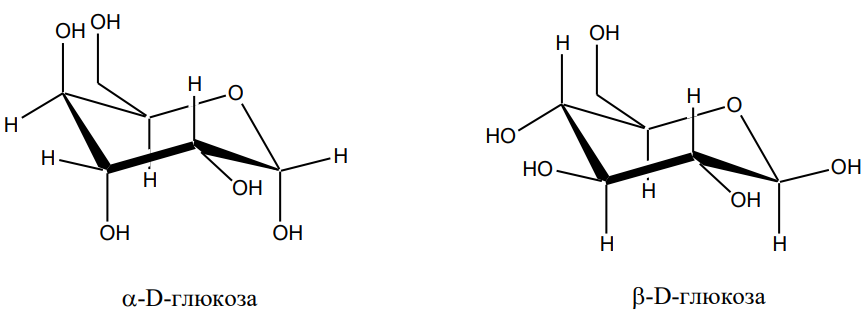
\includegraphics[scale=0.5]{Снимок экрана (666).png}
    \par
\textbf{Рис. 1: }\sffamily{Аномеры D-глюкозы в конформации кресла}.
 \end{center}
\par \vspace{0.5 cm}

\textit{Глюкозооксидазы} (D-глюкозо-1-оксидазы) --- это ферменты различного происхождения, окисляющие $\beta$-D-глюкозу молекулярным кислородом до глюконо-1,5-лактона. В процессе этой трансформации образуется также перекись водорода. \par \vspace{0.2 cm}
Глюкозооксидазы выделены из бактерий, плесневых грибов и т.д. Молекула глюкозооксидазы имеет \textit{четвертичную структуру}. Этот фермент состоит, как правило, из двух субъединиц (\textit{рис. 2}).

\graphicspath{{./images/}}
		\begin{center}
		
			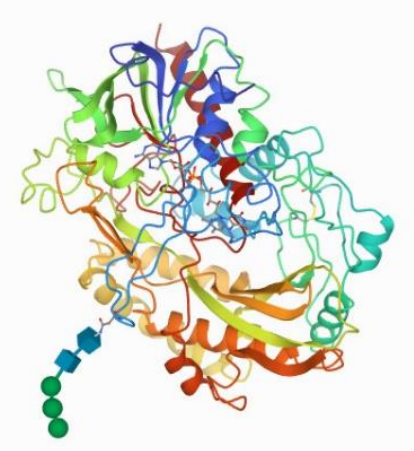
\includegraphics[scale=0.7]{Снимок экрана (667).png}
    \par
\textbf{Рис. 2: }\sffamily{3D-структура глюкозооксидазы плесневого гриба} \textit{Aspergillius Niger}.
 \end{center}
\par \vspace{0.5 cm}

Каждая субъединица содержит одну молекулу \textit{флавинадениндинуклеотидфосфата} (ФАД). Именно этот фрагмент энзима ответственен за окислительно-восстановительные превращения субстратов --- глюкозы (углеводов) и кислорода. 

\graphicspath{{./images/}}
		\begin{center}
		
			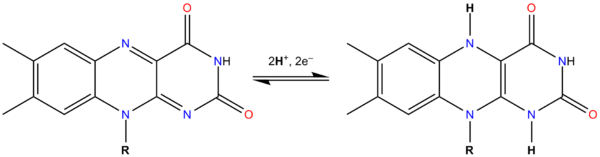
\includegraphics[scale=1]{600px-FAD_FADH2_equlibrium.png}
    \par
\textbf{Рис. 3: }\sffamily{Трансформация ФАД $\Longleftrightarrow{}$ ФАДH$_2$}.
 \end{center}
\par \vspace{0.5 cm}

В процессе трансформации ФАД восстанавливается до ФАДH$_2$, принимая два электрона и два протона. При взаимодействии ФАДH$_2$ с молекулярным кислородом образуется перекпись водорода и регенерируется ФАД в окисленной форме. \par \vspace{0.2 cm}

Ферментативное окисление $\beta$-D-глюкозы до глюконо-1,5-лактона в присутствии глюкозооксидазы протекает с высоко скоростью уже при комнатной температуре (25 $^{\circ}$C):

\graphicspath{{./images/}}
		\begin{center}
		
			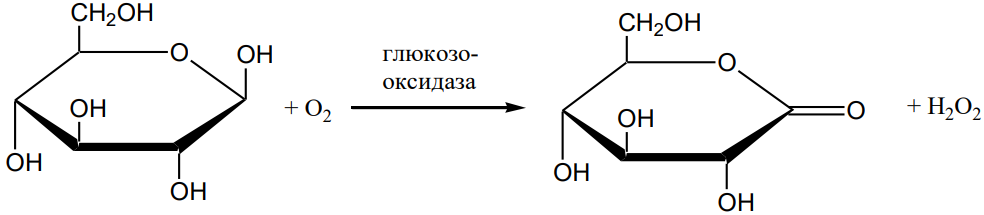
\includegraphics[scale=0.5]{Снимок экрана (668).png}
    \par
\textbf{Рис. 4: }\sffamily{Ферментативное окисление глюкозы до лактона}.
 \end{center}
\par \vspace{0.5 cm}

Образующийся глюконо-1,5-лактон гидролизуется водой в условиях реакции до глюконовой кислоты:

\graphicspath{{./images/}}
		\begin{center}
		
			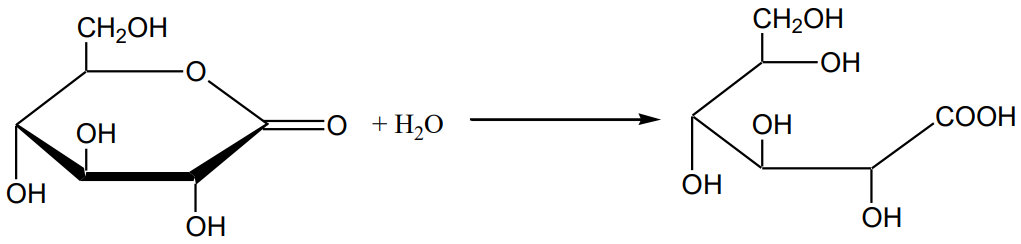
\includegraphics[scale=0.45]{Снимок экрана (669).png}
    \par
\textbf{Рис. 5: }\sffamily{Гидролиз лактона}.
 \end{center}
\par \vspace{0.5 cm}

Постулируется, что реакция протекает по т.н. \textit{пинг-понг}-механизму. Он предполагает постадийность с последовательным присоединением сначала первого субстрата (глюкозы), затем второго (кислорода), без образования тройного фермент-субстратного комплекса:

\graphicspath{{./images/}}
		\begin{center}
		
			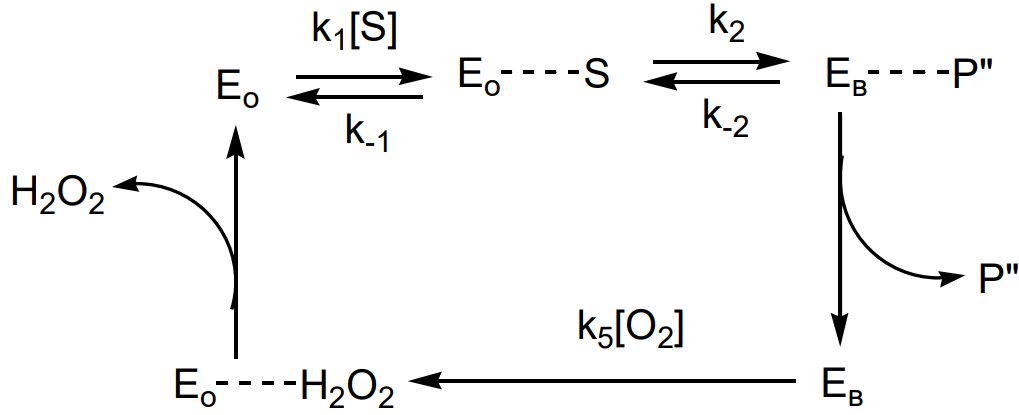
\includegraphics[scale=0.5]{Снимок экрана (670).png}
    \par
\textbf{Рис. 6: }\sffamily{\textit{Пинг-понг}-механизм}.
 \end{center}
\par \vspace{0.5 cm}

где S --- глюкоза, P$^{''}$ --- глюконолактон, E$_{\text{о}}$ --- фермент с коферментом ФАД в окисленной форме, E$_{\text{в}}$ --- фермент с коферментом ФАДH$_2$ в восстановленной форме. \par \vspace{0.2 cm}
Та же схема в упрощенном виде:
\Large
\[
\rm E_{\text{о}} + S \hspace{0.2 cm} {\mbox{\Charrow[30]{rl}{$k_1$}{$k_{-1}$}}} \hspace{0.2 cm} E_{\text{в}}P^{''}
\] \large
\Large
\[
\rm E_{\text{в}}P^{''} \hspace{0.2 cm} {\mbox{\Charrow[30]{r}{$k_3$}{}}} \hspace{0.2 cm} E_{\text{в}} + P^{''}
\] \large
\Large
\[
\rm E_{\text{в}} + O_{2} \hspace{0.2 cm} {\mbox{\Charrow[30]{r}{$k_5$}{}}} \hspace{0.2 cm} E_{\text{о}} + H_2O_2
\] \large
\par \vspace{0.2 cm}
Предполагаем первую стадию рановесной:
\Large
\[
K_1 = \frac{k_1}{k_{-1}} = \frac{[\rm E_{\text{в}}P^{''}]}{[\rm E_{\text{о}}] [\rm S]}
\] \large
\Large
\[
\frac{d[\rm E_{\text{в}}]}{dt} = k_3[\rm E_{\text{в}}P^{''}] - \it k_{\rm 5}[\rm O_2][\rm E_{\text{в}}] \approx 0
\] \large
\Large
\[
[\rm E_{\text{в}}] = \it \frac{k_{\rm 3}[\rm E_{\text{в}}P^{''}]}{k_{\rm 5}[\rm O_2]}
\] \large
\par \vspace{0.2 cm}
Выразим полную концентрацию фермента:
\Large
\[
[\rm E]_0 = [\rm E_{\text{о}}] + [\rm E_{\text{в}}] + [\rm E_{\text{в}}P^{''}] = \frac{[\rm E_{\text{в}}P^{''}]}{\it K_{\rm 1}[\rm S]} + \it \frac{k_{\rm 3}[\rm E_{\text{в}}P^{''}]}{k_{\rm 5}[\rm O_2]} + [\rm E_{\text{в}}P^{''}]
\] \large
\par \vspace{0.2 cm}
Скорость реакции --- скорость образования продукта P$^{''}$:
\Large
\[
w = \frac{d[\rm P^{''}]}{dt} = k_{3}[\rm E_{\text{в}}P^{''}] = \it \frac{k_{\rm 3}[\rm E]_{\rm 0}}{\frac{\rm 1}{\it K_{\rm 1}[\rm S]} + \it \frac{k_{\rm 3}}{k_{\rm 5}[\rm O_2]} + \rm 1} = \it \frac{k_{\rm 3}[\rm E]_{\rm 0}[\rm S]}{\frac{\rm 1}{\it K_{\rm 1}} + \it \left(\frac{k_{\rm 3}}{k_{\rm 5}[\rm O_2]} + \rm 1 \right)[\rm S]}
\] \large
\par \vspace{0.2 cm}
Рассмотрим предельные случаи:
\Large
\begin{itemize}
    \item $\frac{k_3}{k_5[\rm O_2]} \ll 1$: \hspace{0.2 cm} $\it w = \frac{k_{\rm 3}[\rm E]_{\rm 0}[\rm S]}{\frac{\rm 1}{K_{\rm 1}} + [\rm S]}$; \hspace{0.2 cm} $w_{max} = k_{3}[\rm E]_{\rm 0}$

    \item $\frac{k_3}{k_5[\rm O_2]} \gg 1$: \hspace{0.2 cm} $\it w = \frac{k_{\rm 5}[\rm E]_{\rm 0}[\rm O_2][\rm S]}{\frac{k_{\rm 5}[\rm O_2]}{k_{\rm 3}K_{\rm 1}} + [\rm S]}$; \hspace{0.2 cm} $w_{max} = k_{5}[\rm E]_{\rm 0}[O_2]$
\end{itemize} \large
\par \vspace{0.2 cm}
Если принять, что концентрация кислорода постоянна, то оба уравнения по форме совпадают с классическим уравнением Михаэлиса --- Ментен для односубстратной реакции.
 

\section{\LARGE \textbf{Методика измерений}}
\par \hspace{0.33 cm}
Запись кинетических кривых проводится на спектрофотометре Solar (время съемки --- 15 мин, шаг --- 1 с) на 390 нм. С помощью термостата устанавливается температура 30$^{\circ}$C. Для каждого углевода кинетика записывается 2 раза. Методика приготовления рабочего раствора в кювете описана в следующем пункте. Здесь отдельно отметим, что \textbf{\sffamily{очень важно достичь равномерного распределения фермента по раствору}}. \par \vspace{0.2 cm}
Выделившаяся в результате ферментативной реакции перекись водорода взаимодействует с I-реактивом с образованием трийодид-аниона:
\Large
\[
\rm H_2O_2 + 3I^{-} + 2H^{+} \longrightarrow 2H_2O + I_3^{-}
\] \large
\par \vspace{0.1 cm}
Трийодид обладает обладает интенсивным поглощением в ближней УФ-области. В максимуме линии поглощения при 350 нм коэффициент экстинкции $\varepsilon = 2.5 \cdot 10^4$ $\frac{\text{л}}{\text{моль} \cdot \text{см}}$, а при 390 нм $\varepsilon \approx 3 \cdot 10^3$ $\frac{\text{л}}{\text{моль} \cdot \text{см}}$. Результаты измерений записываются в таблицу.


\section{\LARGE \textbf{Используемое оборудование и материалы}}
\par \hspace{0.33 cm}
\textbf{\sffsamily{Оборудование и лабораторное стекло:}}
    \begin{itemize}
        \item мерная колба на 250 мл -- 1 шт.;
        \item стакан на 250 мл -- 1 шт.;
        \item стаканчики на 25 мл -- 4 шт.;
        \item pH-метр;
        \item $\rm UV\text{-}VIS$ спектрофотометр или анлогичный;
        \item кварцевая кювета толщиной 1 см;
        \item автоматические пипетки на 20 мкл;
        \end{itemize}  
\par \vspace{0.3 cm}

\textbf{\sffsamily{Реактивы:}}
    \begin{itemize}
        \item набор углеводов;
        \item дигидрофосфат калия;
        \item кали йодистый;
        \item раствор молибдата натрия (9\%);
        \item раствор $\rm NaOH$ (0.1 M);
        \item раствор глюкозооксидазы (хранится в холодильнике);
        \item стандартный раствор с известным pH --- для калибровки pH-метра;
        \end{itemize}  
\par \vspace{0.3 cm}

\boxed{1} \hspace{0.1 cm} \textbf{\sffamily{Приготовление 0.05 М фосфатного буфера pH 6.0}}: \normalfont \par \vspace{0.1 cm}
Перед началом опыта pH-метр проверяется по стандартному раствору с известным pH (25$^{\circ}$C). 1.71 г дигидрофосфата калия растворяются в 200 мл воды в химическом стакане. pH полученного буферного раствора доводится 1 M $\rm NaOH$ до значения 6.0. Содержимое стакана переносят в мерную колбу на 250 мл и доводят до метки дистиллированной водой. 
\par \vspace{0.5 cm}

\boxed{2} \hspace{0.1 cm} \textbf{\sffamily{Приготовление реактива йодида (I-реактив)}}: \normalfont \par \vspace{0.1 cm}
0.83 г йодида калия растворяются в 8 мл буферного раствора pH 6.0, добавляются 2 мл 9\% раствора молибдата натрия, полученный раствор перемешивается. $\rm KI$-реактив готовится непосредственно перед опытом и использоваться в течение одного занятия.
\par \vspace{0.5 cm}

\boxed{3} \hspace{0.1 cm} 
\textbf{\sffamily{Приготовление 10\% растворов углеводов}}: \normalfont \par \vspace{0.1 cm}
0.5 г углевода (ксилозы, маннозы или глюкозы) растворяются в 5 мл буферного раствора pH 6.0. \par \vspace{0.5 cm}

\boxed{4} \hspace{0.1 cm}
\textbf{\sffamily{Рабочий раствор}} \normalfont для измерения скорости ферментативной реакции готовится непосредственно в кювете спектрофотометра. Для этого в кювете смешиваются приготовленные заранее реагенты (0.5 мл I-реактива, 0.4 мл раствора углевода, 1.1 мл буферного раствора + \textit{20 мкл фермента при интенсивном перемешивании}). \par \vspace{1.5 cm}



\section{\LARGE Результаты измерений}

\graphicspath{{./images/}}
		\begin{center}
		
			\includegraphics[scale=0.7]{нуль.png}
    \par
\textbf{Рис. 7: }\sffamily{Базовая линия (буферный раствор)}.
 \end{center}
\par \vspace{0.5 cm}

\newpage
\subsection{\Large Первичные данные}

\graphicspath{{./images/}}
		\begin{center}
		
			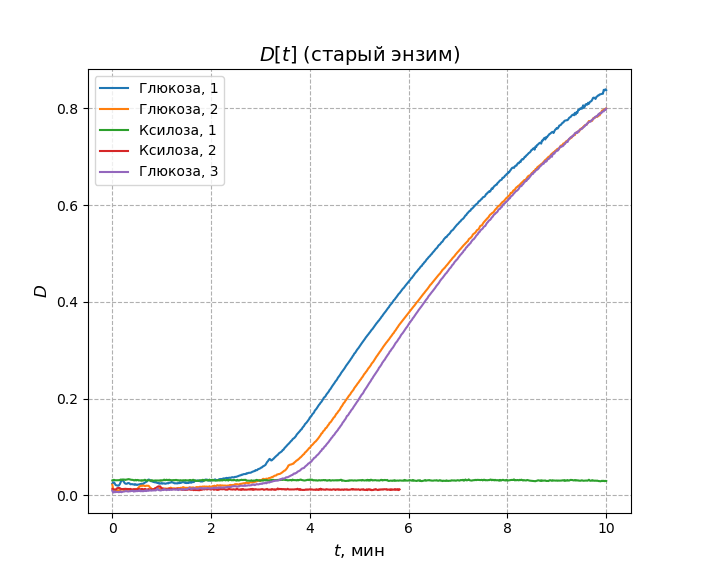
\includegraphics[scale=0.7]{старый энзим.png}
    \par
\textbf{Рис. 8: }\sffamily{Зависимости оптических плотностей растворов от времени (старый энзим)}.
 \end{center}
\par \vspace{0.5 cm}

\graphicspath{{./images/}}
		\begin{center}
		
			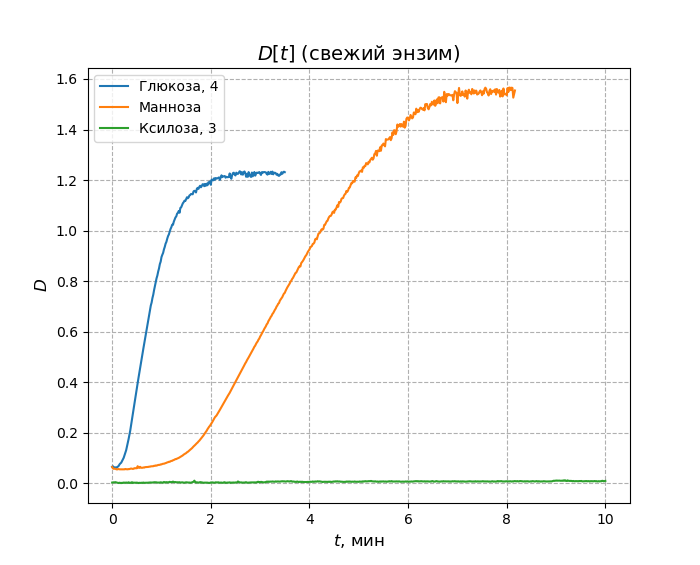
\includegraphics[scale=0.7]{свежий энзим.png}
    \par
\textbf{Рис. 9: }\sffamily{Зависимости оптических плотностей растворов от времени \par (использован свежий энзим)}.
 \end{center}
\par \vspace{0.5 cm}

\graphicspath{{./images/}}
		\begin{center}
		
			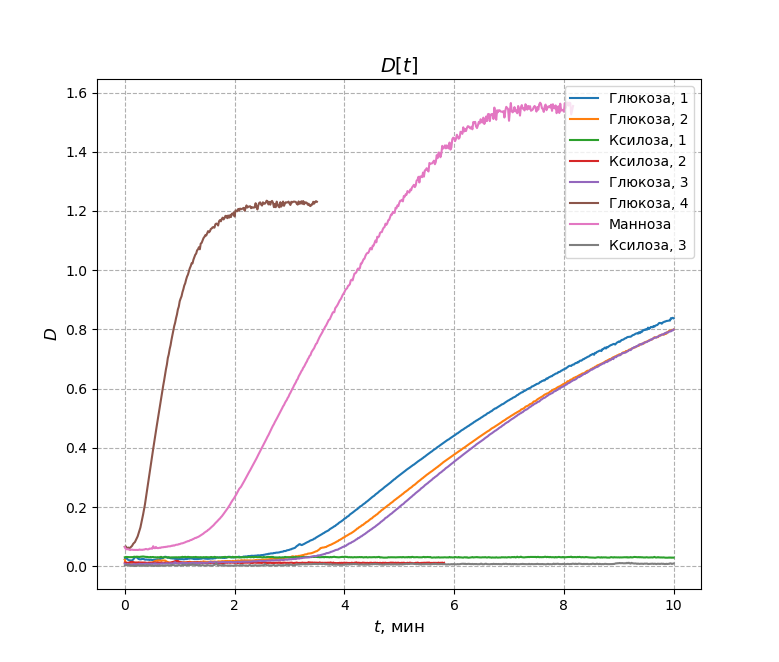
\includegraphics[scale=0.8]{полные данные.png}
    \par
\textbf{Рис. 10: }\sffamily{Полный набор полученных первичных данных}.
 \end{center}
\par \vspace{0.5 cm}


\section{\LARGE Обработка данных}
\par \hspace{0.33 cm}
Для сравнения активностей субстратов в реакции ферментативного окисления оценим максимальные скорости реакций, достигаемые на начальных участках полученных зависимостей. \par
Подберем эмпирические формулы для начальных участков кривых, соответствующих реакциям с участием глюкозы и маннозы, в следующем виде (параметры $D_0$, $D_{\infty}$, $\tau_0$, $T$ определим численно):
\Large
\[
D(t) = D_0 + D_{\infty} \int\limits_{-\infty}^{t}\frac{1}{\sqrt{2\pi T^2}} e^{-\frac{(\tau - \tau_0)^2}{2 T^2}}d\tau \] \large
\par

Все данные для ксилозы аппроксимируем линейными зависимостями.

\graphicspath{{./images/}}
		\begin{center}
		
			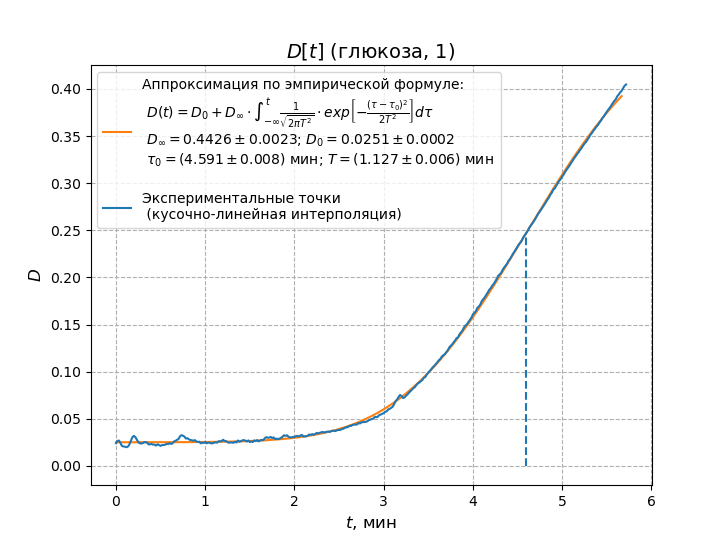
\includegraphics[scale=0.8]{глюкоза_1.png}
    \par
\textbf{Рис. 11: }\sffamily{Начальный участок зависимости $D(t)$ (глюкоза, первое измерение)}.
 \end{center}
\par \vspace{0.5 cm}

\graphicspath{{./images/}}
		\begin{center}
		
			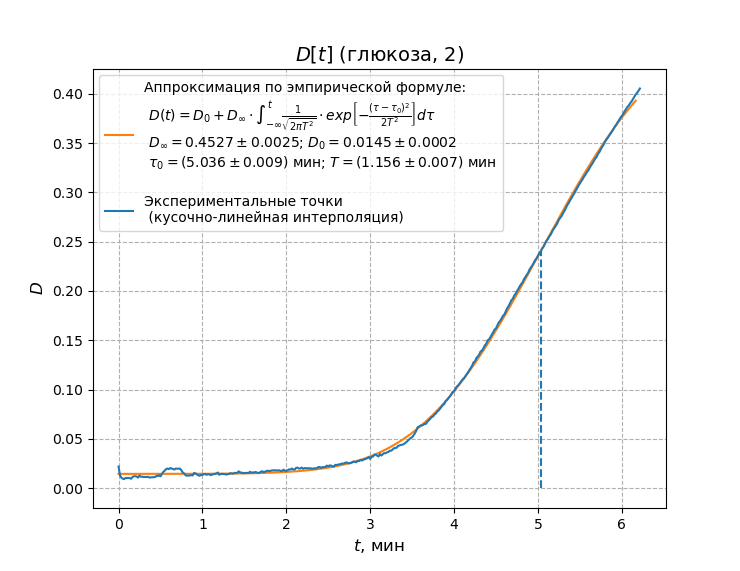
\includegraphics[scale=0.8]{глюкоза_2.png}
    \par
\textbf{Рис. 12: }\sffamily{Начальный участок зависимости $D(t)$ (глюкоза, второе измерение)}.
 \end{center}
\par \vspace{0.5 cm}

\graphicspath{{./images/}}
		\begin{center}
		
			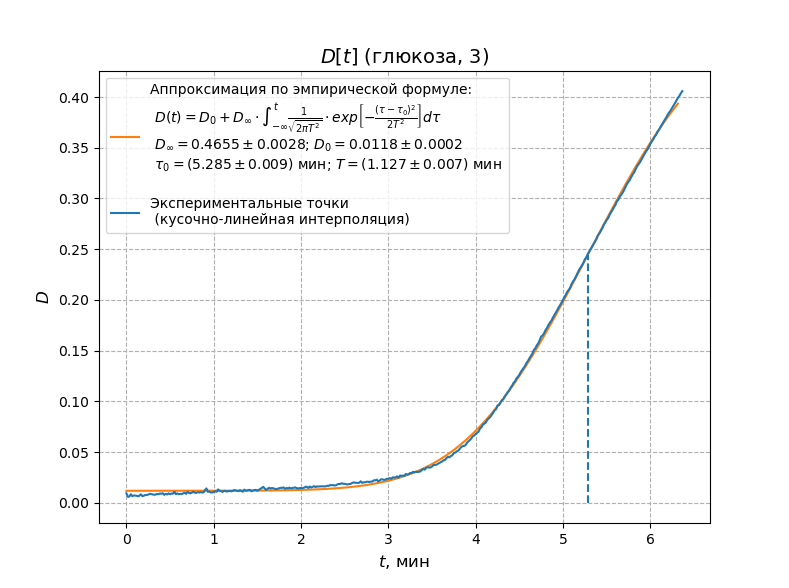
\includegraphics[scale=0.75]{глюкоза_3.png}
    \par
\textbf{Рис. 13: }\sffamily{Начальный участок зависимости $D(t)$ (глюкоза, третье измерение)}.
 \end{center}
\par \vspace{0.5 cm}

\graphicspath{{./images/}}
		\begin{center}
		
			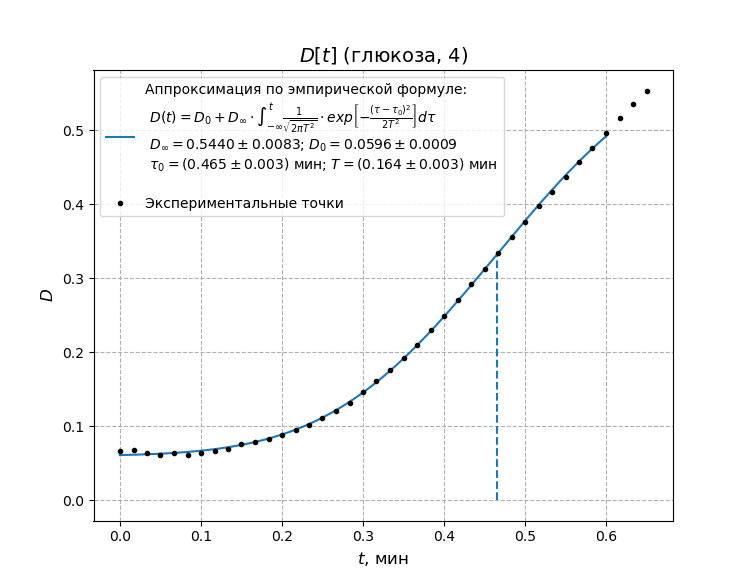
\includegraphics[scale=0.75]{глюкоза_4.png}
    \par
\textbf{Рис. 14: }\sffamily{Начальный участок зависимости $D(t)$ (глюкоза, четвертое измерение)}.
 \end{center}
\par \vspace{0.5 cm}

\graphicspath{{./images/}}
		\begin{center}
		
			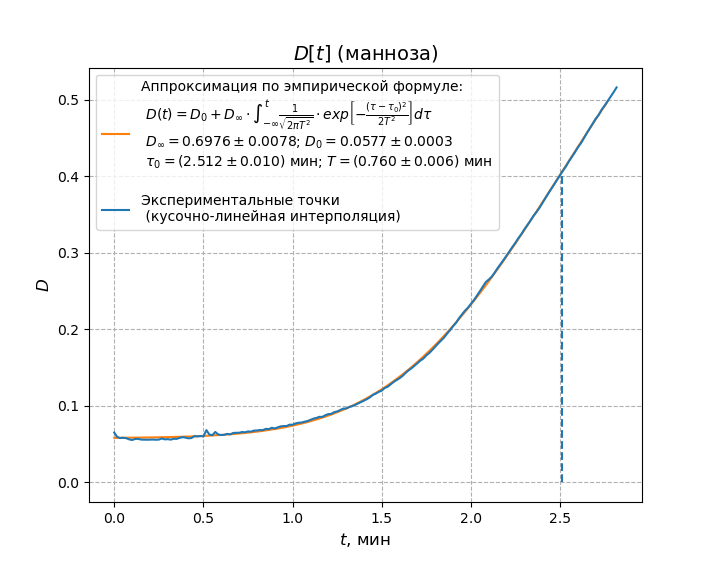
\includegraphics[scale=0.8]{манноза.png}
    \par
\textbf{Рис. 15: }\sffamily{Начальный участок зависимости $D(t)$ (манноза)}.
 \end{center}
\par \vspace{0.5 cm}

\graphicspath{{./images/}}
		\begin{center}
		
			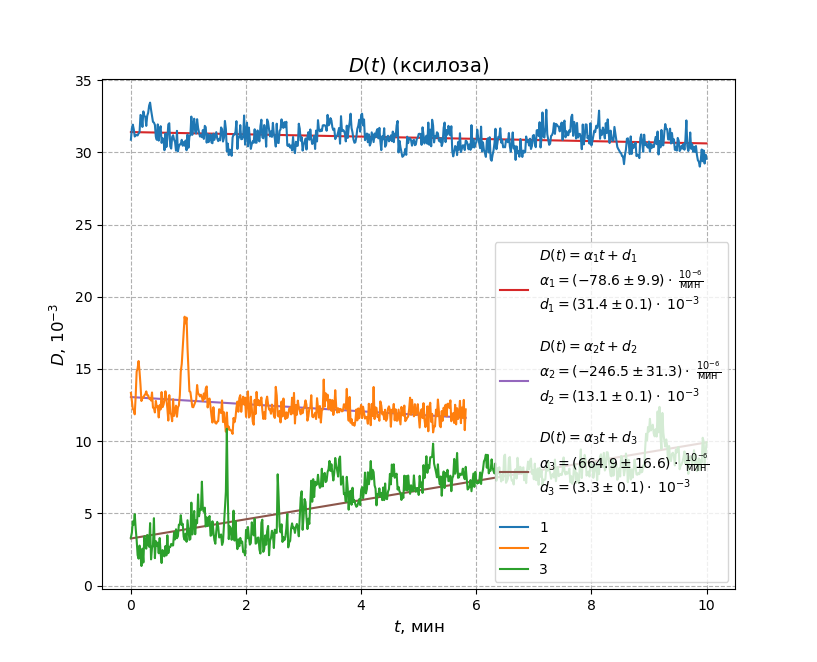
\includegraphics[scale=0.7]{ксилоза.png}
    \par
\textbf{Рис. 16: }\sffamily{Зависимости $D(t)$ для реакционных смесей с участием ксилозы, аппроксимированные линейными законами}.
 \end{center}
\par \vspace{0.5 cm}

Считая известными коэффициент экстинкции $\varepsilon = 3 \cdot 10^3$ $\frac{\text{л}}{\text{моль} \cdot \text{см}}$ и толщину кюветы $l = 1$ см, а основании данных о временных зависимостях оптических плотностей оценим зависимость скорости образования трийодид-иона от времени: $\frac{d[\rm I_3^{-}]}{dt} = \frac{1}{\varepsilon l} \frac{dD}{dt}$.

\graphicspath{{./images/}}
		\begin{center}
		
			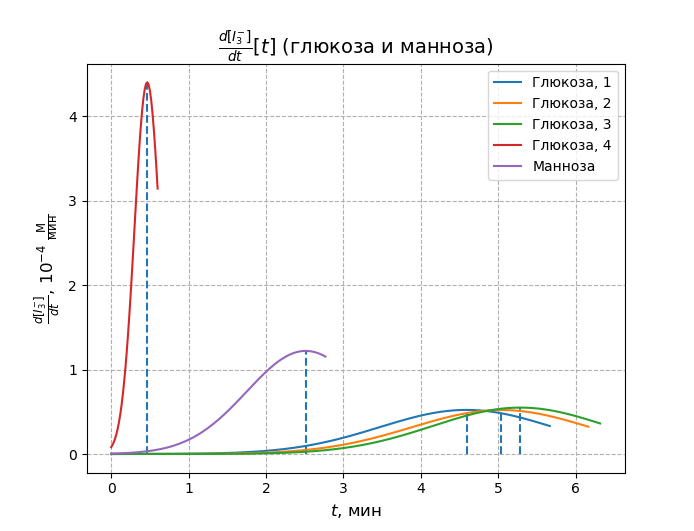
\includegraphics[scale=0.85]{скорости реакций.png}
    \par
\textbf{Рис. 17: }\sffamily{Зависимости скоростей образования трийодида от времени --- функции Гаусса (пунктиром отмечены максимумы)}.
 \end{center}
\par \vspace{0.5 cm}

Приведем максимальные значения скоростей:
\par \vspace{0.2 cm}

\begin{center}
\textbf{Таблица 2.} \sffamily{Максимальные скорости образования трийодид-иона \par в опытах с участием глюкозы и маннозы}. \normalfont

\vspace{0.3cm}
\begin{tabular}{|c|c|c|c|c|c|c|c|c|}
    \hline
    Опыт & Глюкоза, 1 & Глюкоза, 2 & Глюкоза, 3 & Глюкоза, 4 & Манноза\\
    \hline
    $\left( \frac{d[\rm I_3^{-}]}{dt} \right)_{max}$, 10$^{-4}$ $\frac{\text{M}}{\text{мин}}$ & 0.522 $\pm$ 0.004 & 0.521 $\pm$ 0.004 & 0.549 $\pm$ 0.005 & 4.4 $\pm$ 0.1 & 1.22 $\pm$ 0.02 \\
    \hline

\end{tabular}
\end{center}

\par \vspace{0.2 cm}
\begin{itemize}
    \item Среднее по первым трем опытам: $(5.307 \pm 0.025) \cdot 10^{-5}$ $\frac{\text{M}}{\text{мин}}$
\end{itemize}
\par \vspace{0.2 cm}

Наконец, воспользуемся тем, что $\frac{d[\rm I_3^{-}]}{dt} = \frac{d[\rm H_2O_2]}{dt}$ и представим скорость реакции в виде величины $\frac{V_{\Sigma}}{N_{\text{мкл}}[V_{\text{р-ра}}(GOx)]} \left( \frac{d[\rm H_2O_2]}{dt} \right)_{max}$, где $V_{\Sigma}$ --- полный объем раствора в кювете, $N_{\text{мкл}}[V_{\text{р-ра}}(GOx)]$ --- число добавленных микролитров раствора энзима (глюкозоосидазы). Представим полученные результаты в виде таблиц со значениями этой скорости и относительных активностей субстратов (отношений скоростей к соответствующим максимальным значениям).

\newpage
\begin{center}
\textbf{Таблица 3.} \sffamily{Скорости реакций и относительные активности субстратов \par при использовании старого энзима}. \normalfont

\vspace{0.3 cm}
\begin{tabular}{|c|c|c|c|c|c|c|c|c|}
    \hline
    Опыт & Глюкоза (среднее) & Ксилоза, 1--2\\
    \hline
    $\frac{V_{\Sigma}}{N_{\text{мкл}}[V_{\text{р-ра}}(GOx)]} \left( \frac{d[\rm H_2O_2]}{dt} \right)_{max}$, $\frac{\text{моль}}{\text{мин}}$ & (5.307 $\pm$ 0.025) $\cdot$ 10$^{-9}$  & $\sim$ 0 (более точная оценка невозможна)\\
    \hline
    Отн. активность, \% & 100 & $\sim$ 0 \\
    \hline

\end{tabular}
\end{center}
\par \vspace{0.2 cm}

\begin{center}
\textbf{Таблица 4.} \sffamily{Скорости реакций и относительные активности субстратов \par при использовании \textit{свежего} энзима}. \normalfont

\vspace{0.3 cm}
\begin{tabular}{|c|c|c|c|c|c|c|c|c|}
    \hline
    Опыт & Глюкоза, 4 & Ксилоза, 3 & Манноза \\
    \hline
    $\frac{V_{\Sigma}}{N_{\text{мкл}}[V_{\text{р-ра}}(GOx)]} \left( \frac{d[\rm H_2O_2]}{dt} \right)_{max}$, $\frac{\text{моль}}{\text{мин}}$ & (4.4 $\pm$ 0.1) $\cdot$ 10$^{-8}$ & (2.22 $\pm$ 0.06) $\cdot$ 10$^{-11}$ & (1.22 $\pm$ 0.02) $\cdot$ 10$^{-8}$ \\
    \hline
    Отн. активность, \% & 100 & 0.05 & 27.7 $\pm$ 0.7 \\
    \hline

\end{tabular}
\end{center}
\par \vspace{1 cm}

\section{\LARGE Выводы}
\par \hspace{0.33 cm}

По результатам измерений, как и ожидалось, была выявлена специфичность глюкозооксидазы к глюкозе, что видно по оцененным величинам скоростей соответствующих реакций: при использовании в качестве субстратов ксилозы и маннозы скорости падали до $\sim$30\% и $\sim$0\% соответственно, считая от уровня скорости с субстратом --- глюкозой. \par \vspace{0.2 cm}
В условиях опыта было выявлено интересное явление --- наличие у всех реакций некоторого варьирующегося инкубационного периода, когда реакци практически не идет, с более или менее плавным переходом к пику скорости реакции. Затем, как и ожидалось, наблюдается спад скорости. В данной работе начальные участки кинетических кривых были приближены с помощью эмпирической формулы, вид которой позволил оценить время достижения максимальной скорости реакции и само значение скорости в максимуме. \par \vspace{0.2 cm}
Наличие инкубационного периода во всех данных, в том числе при применении свежеприготовленного энзима, может быть связано, например, с недостаточным количеством молибдат-ионов в растворе. Данная гипотеза требует экспериментальной проверки.

\end{document}	
